\subsection{Overview of System Approach}

\begin{figure}[H]
    \vspace{1em} 
    \centering
    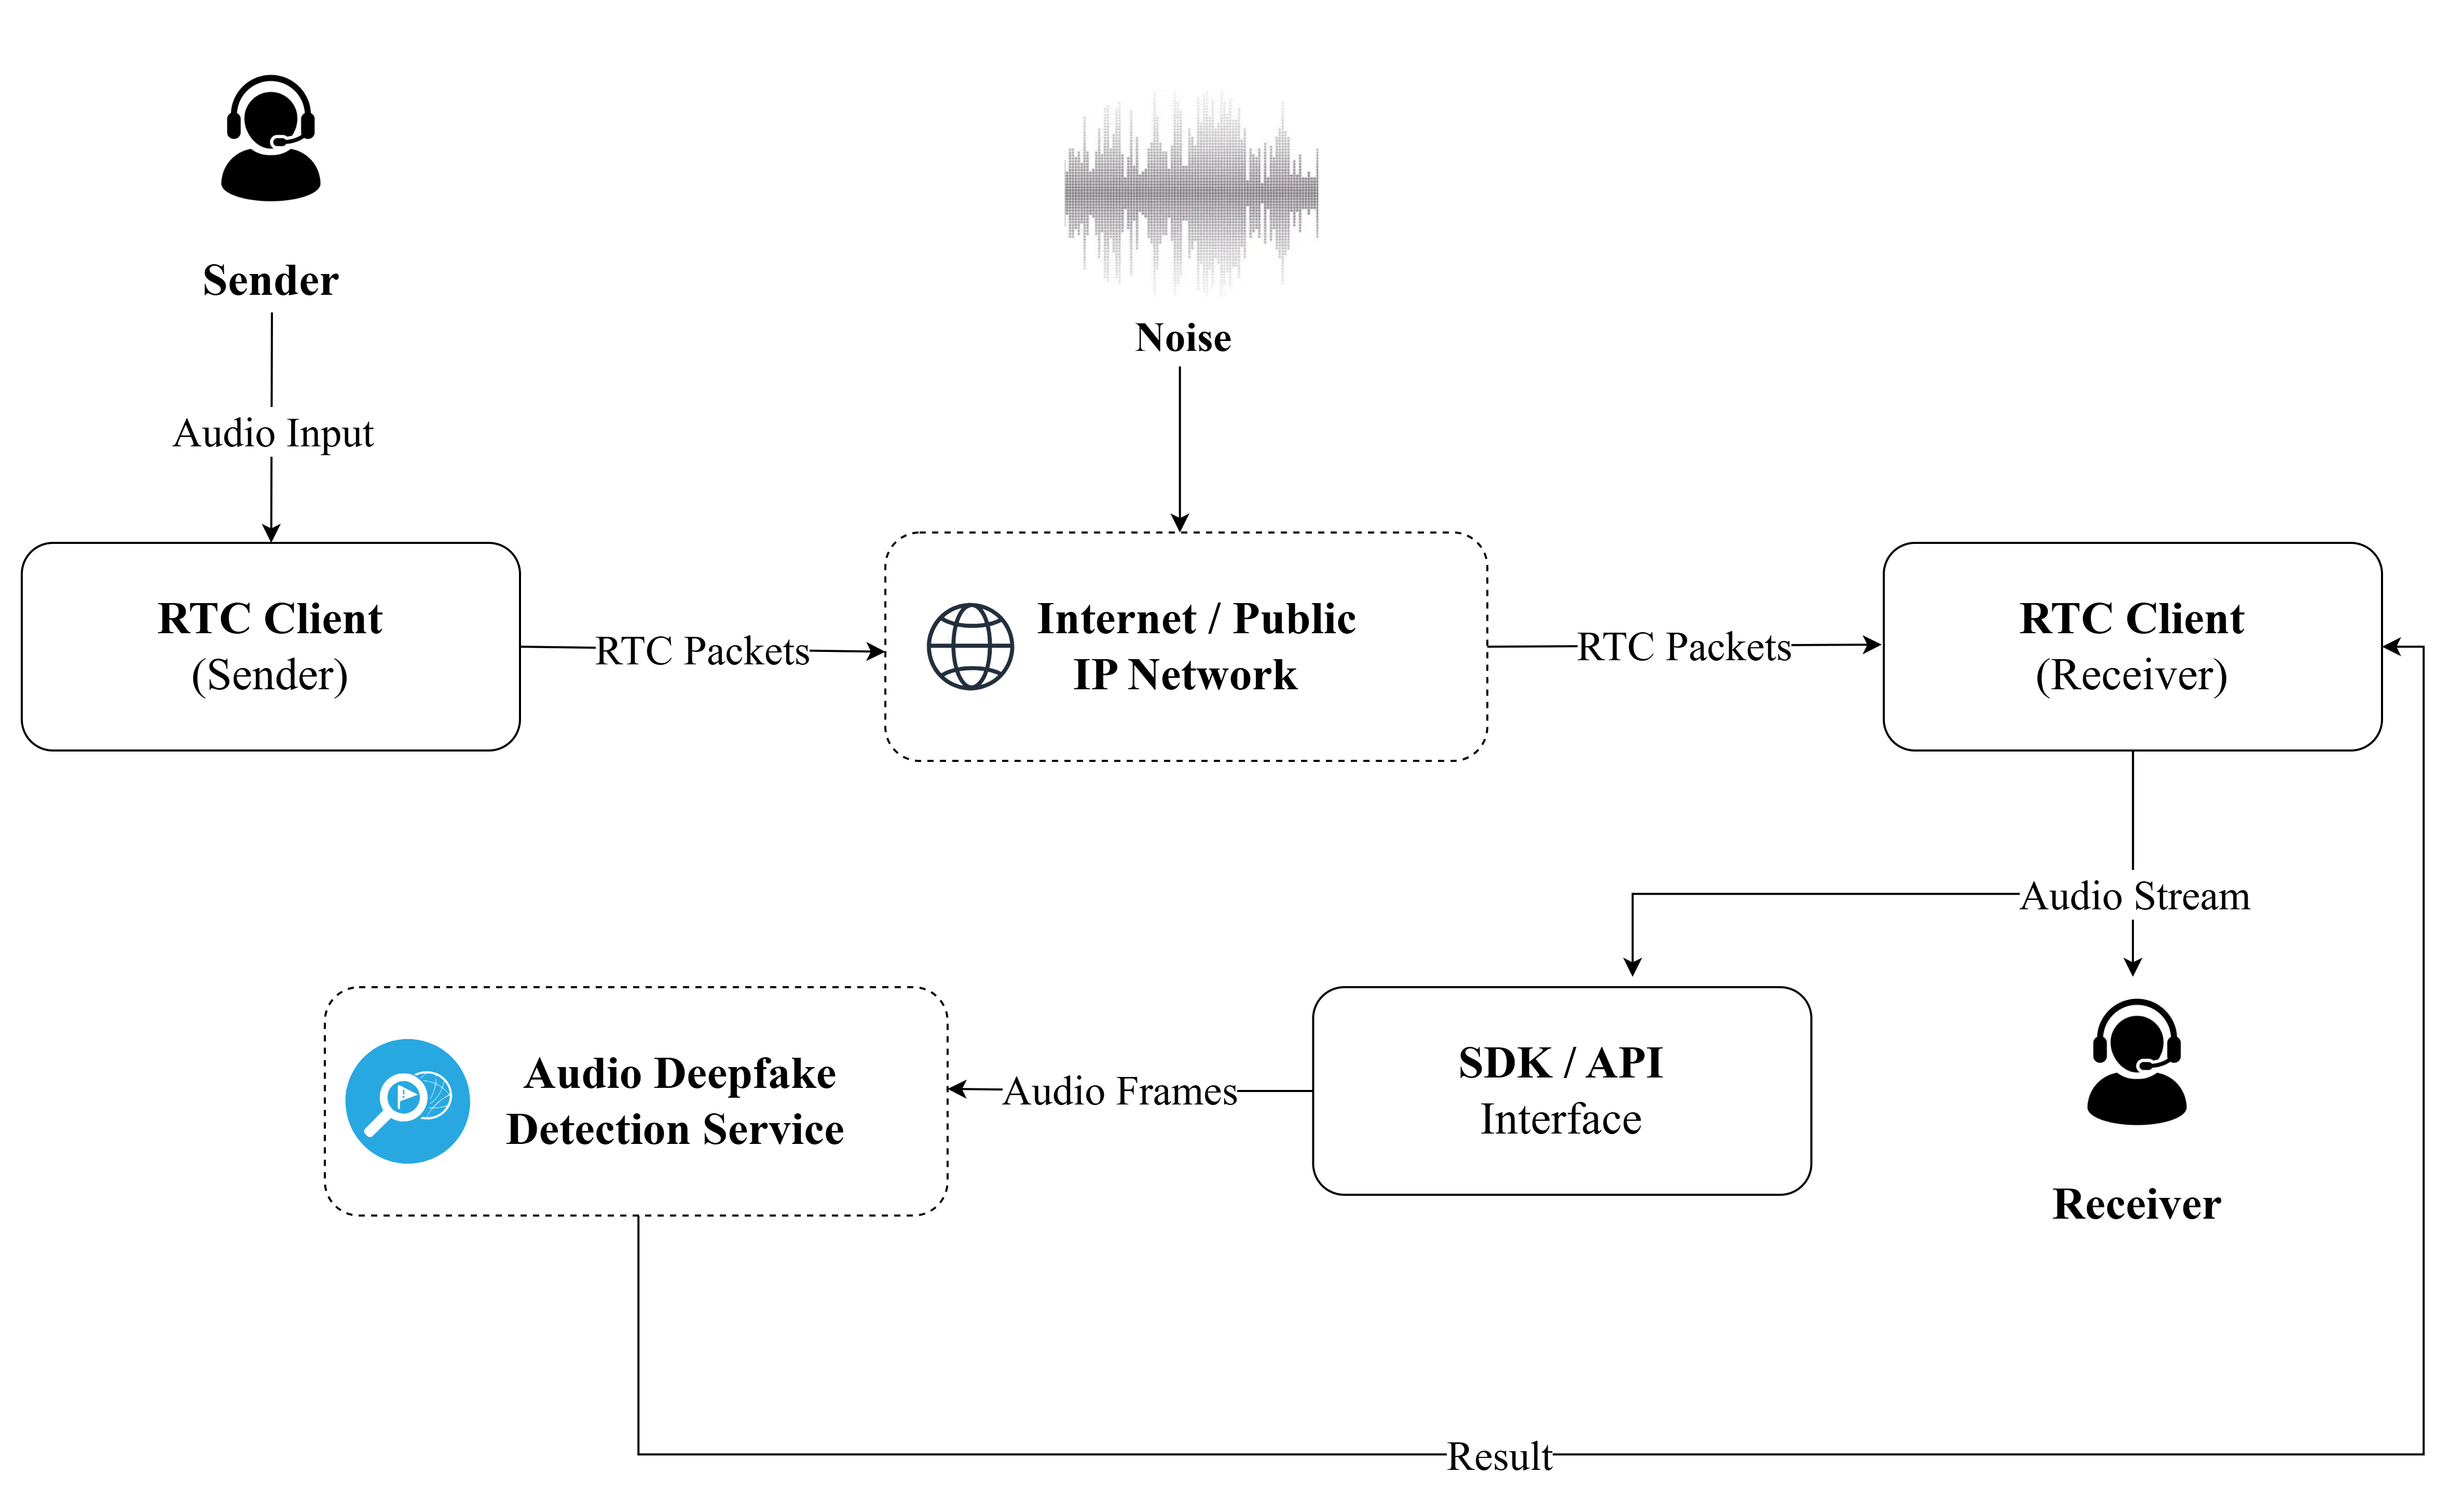
\includegraphics[width=1\textwidth]{images/methodology/system_block_diagram.jpg}
    \vspace{0.25cm}
    \caption{High-Level System Block Diagram}
    \label{fig:system_block_diagram}
\end{figure}

The proposed framework is a real-time audio deepfake detection system integrated into RTC/VoIP communication pipelines as an external service layer. The system is deliberately structured as a decoupled architecture, where the RTC communication stack and the detection system operate independently but are connected through an audio streaming interface.

This design is necessary because real-world RTC platforms (Zoom-like systems, WebRTC-based applications, VoIP services) are closed systems with proprietary encoding, packet handling, and audio enhancement pipelines. Therefore, the detection mechanism cannot be embedded directly into the sender-side or receiver-side application logic. The system is composed of four interacting subsystems:

\begin{enumerate}
    \item Sender Side (RTC Client)
    \item Network Transmission Layer
    \item Receiver Side (RTC Client)
    \item Audio Deepfake Detection Service (External Plugin Layer)
\end{enumerate}

